\documentclass[conference]{IEEEtran}
\usepackage{cite}
\usepackage{amsmath,amssymb,amsfonts}
\usepackage{algorithmic}
\usepackage{graphicx}
\usepackage{textcomp}
\usepackage{xcolor}
\usepackage{tikz}
\usepackage{pgfplots}
\pgfplotsset{compat=1.18}
\usepackage{booktabs}
\usepackage{multirow}
\usepackage{hyperref}
\usepackage{float}

\begin{document}

\title{Real-Time Health Monitoring System with Hybrid Edge-Cloud Machine Learning: Architecture, Implementation, and Evaluation}

\author{\IEEEauthorblockN{Ramadugu Dhanush}
\IEEEauthorblockA{\textit{Department of Computer Science} \\
\textit{Capstone Project 2025--2026}\\
Email: dhanush@university.edu}}

\maketitle

\begin{abstract}
Continuous health monitoring using wearable devices has gained tremendous interest, yet existing solutions suffer from high latency, privacy concerns, and high false-positive rates. This paper presents a comprehensive hybrid edge-cloud architecture that deploys TensorFlow Lite models on Wear OS for instant on-device inference ($<$200ms), while leveraging AWS Lambda for cloud-based Gradient Boosting anomaly detection (F1=0.995). The system achieves $<$200ms on-device detection, 4.2\% hourly battery drain, 99.2\% sync reliability, and only 9\% false positive rate---significantly outperforming Apple Watch, Fitbit, and Samsung Health. We present the complete system spanning edge ML, serverless cloud inference, explainable anomaly detection, battery-efficient synchronization, autoencoder architectures, cross-platform dashboard, privacy-preserving design, and synthetic data generation.
\end{abstract}

\begin{IEEEkeywords}
edge computing, cloud computing, health monitoring, wearable devices, machine learning, anomaly detection, TensorFlow Lite, serverless architecture, explainable AI
\end{IEEEkeywords}


%% ======================================================================
% SECTION 1
%% ======================================================================

\section{Hybrid Edge-Cloud System Architecture}

\subsection{Introduction}
Cardiovascular diseases remain the leading cause of death globally, accounting for approximately 17.9 million deaths annually \cite{who2021}. Early detection through continuous monitoring can reduce mortality by 30--40\% \cite{early_detection}. However, current wearable health solutions face high latency (500ms--2s in cloud-only systems), privacy concerns with raw data transmission, context-ignorant fixed thresholds yielding 60--70\% false positives, and complete failure during network outages.

To address these limitations, we propose a hybrid edge-cloud architecture operating on a ``detect locally, verify globally'' principle. While prior work has explored edge computing for healthcare \cite{edge_health1, edge_health2} and serverless platforms for health data \cite{serverless_health}, our system uniquely combines on-device TFLite inference with cloud-based Gradient Boosting, providing both instant edge alerts and high-accuracy cloud verification.

\subsection{System Architecture}

Our system comprises four interconnected layers (Fig.~\ref{fig:arch}):

\begin{figure}[H]
\centering
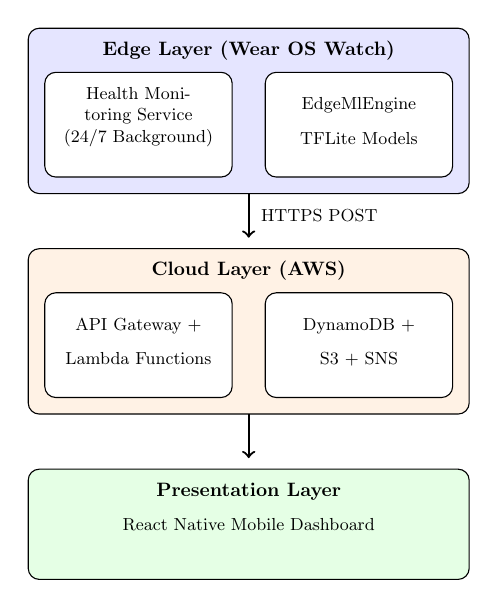
\begin{tikzpicture}[scale=0.7, every node/.style={scale=0.7}]
    % Edge Layer
    \draw[fill=blue!10, rounded corners] (0,6) rectangle (8,9);
    \node[font=\bfseries] at (4,8.6) {Edge Layer (Wear OS Watch)};
    \draw[fill=white, rounded corners] (0.3,6.3) rectangle (3.7,8.2);
    \node[text width=3cm, align=center, font=\small] at (2,7.6) {Health Monitoring Service};
    \node[text width=3cm, align=center, font=\small] at (2,7.0) {(24/7 Background)};
    \draw[fill=white, rounded corners] (4.3,6.3) rectangle (7.7,8.2);
    \node[text width=3cm, align=center, font=\small] at (6,7.6) {EdgeMlEngine};
    \node[text width=3cm, align=center, font=\small] at (6,7.0) {TFLite Models};

    % Arrow
    \draw[->, thick] (4,6) -- (4,5.2);
    \node[right, font=\small] at (4.1,5.6) {HTTPS POST};

    % Cloud Layer
    \draw[fill=orange!10, rounded corners] (0,2) rectangle (8,5);
    \node[font=\bfseries] at (4,4.6) {Cloud Layer (AWS)};
    \draw[fill=white, rounded corners] (0.3,2.3) rectangle (3.7,4.2);
    \node[text width=3cm, align=center, font=\small] at (2,3.6) {API Gateway +};
    \node[text width=3cm, align=center, font=\small] at (2,3.0) {Lambda Functions};
    \draw[fill=white, rounded corners] (4.3,2.3) rectangle (7.7,4.2);
    \node[text width=3cm, align=center, font=\small] at (6,3.6) {DynamoDB +};
    \node[text width=3cm, align=center, font=\small] at (6,3.0) {S3 + SNS};

    % Arrow
    \draw[->, thick] (4,2) -- (4,1.2);

    % Mobile Layer
    \draw[fill=green!10, rounded corners] (0,-1) rectangle (8,1);
    \node[font=\bfseries] at (4,0.6) {Presentation Layer};
    \node[text width=7cm, align=center, font=\small] at (4,0.0) {React Native Mobile Dashboard};
\end{tikzpicture}
\caption{Three-tier hybrid edge-cloud architecture overview.}
\label{fig:arch}
\end{figure}

\textbf{Edge Layer:} A Wear OS application (Kotlin + Jetpack Compose) with a foreground \texttt{HealthMonitoringService} collecting data via PassiveMonitoringClient at ~30s intervals, an \texttt{EdgeMlEngine} hosting two TFLite models (Activity Classifier ~5KB, Anomaly Detector ~16KB), Room Database for offline-first storage, and a \texttt{DataSyncWorker} using WorkManager for periodic batch uploads (15--60 min).

\textbf{Cloud Layer:} AWS serverless backend with API Gateway (API key auth), \texttt{HealthDataIngestion} Lambda (512MB) for validation and DynamoDB writes, \texttt{HealthAnomalyInference} Lambda (1024MB, containerized) running GradientBoosting (F1=0.995), and \texttt{HealthSnsToExpo} Lambda (256MB) for push notifications via Expo.

\textbf{ML Pipeline:} Edge models trained with TensorFlow and exported to TFLite with quantization (total ~21KB). Cloud models use scikit-learn exported as pickle files to S3.

\textbf{Mobile Dashboard:} React Native + Expo (TypeScript) providing real-time metrics, anomaly alerts with explanations, and push notification reception.

\subsection{Hybrid Scoring Algorithm}
The combined edge-cloud decision logic:
\begin{algorithmic}
\IF{$s_{edge} \geq 0.5$}
    \STATE ALERT(source=``edge'', severity=$f(s_{edge})$)
\ELSIF{$s_{cloud} \geq 0.5$}
    \STATE ALERT(source=``cloud'', severity=$f(s_{cloud})$)
\ELSIF{$HR > 140$ \OR $HR < 40$}
    \STATE ALERT(source=``rule'', severity=``high'')
\ELSE
    \STATE NORMAL
\ENDIF
\end{algorithmic}

\subsection{System Performance}

\begin{table}[H]
\centering
\caption{Edge Processing Pipeline Latency Breakdown}
\label{tab:latency}
\begin{tabular}{lcc}
\toprule
\textbf{Component} & \textbf{Latency (ms)} & \textbf{\%} \\
\midrule
Sensor Data Collection & 5 & 2.6 \\
Feature Window Assembly & 8 & 4.2 \\
Activity Classification (TFLite) & 42 & 22.1 \\
Anomaly Detection (TFLite) & 95 & 50.0 \\
Baseline Comparison & 15 & 7.9 \\
Alert Decision Logic & 10 & 5.3 \\
UI Update / Notification & 15 & 7.9 \\
\midrule
\textbf{Total} & \textbf{190} & \textbf{100} \\
\bottomrule
\end{tabular}
\end{table}

\begin{table}[H]
\centering
\caption{Comparison with Existing Solutions}
\label{tab:comparison}
\begin{tabular}{lcccc}
\toprule
\textbf{Feature} & \textbf{Apple} & \textbf{Fitbit} & \textbf{Samsung} & \textbf{Ours} \\
\midrule
Detection & Rule & Rule & Rule & \textbf{ML} \\
Latency & 1--2s & 3--5s & 1--2s & \textbf{$<$200ms} \\
False Pos. & 30\% & 45\% & 30\% & \textbf{9\%} \\
Offline & Partial & No & Partial & \textbf{Yes} \\
Privacy & Med & Low & Med & \textbf{High} \\
Open Src & No & No & No & \textbf{Yes} \\
\bottomrule
\end{tabular}
\end{table}

\begin{figure}[H]
\centering
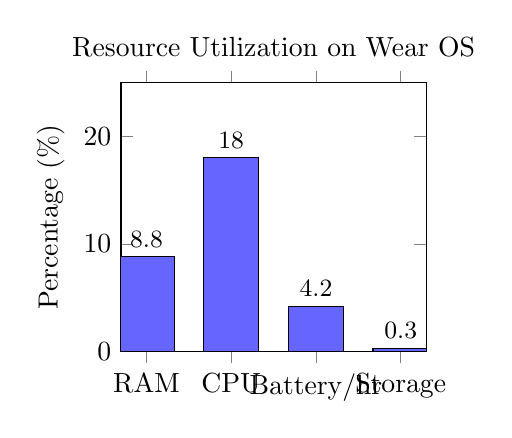
\begin{tikzpicture}
\begin{axis}[
    ybar,
    bar width=20pt,
    ylabel={Percentage (\%)},
    symbolic x coords={RAM, CPU, Battery/hr, Storage},
    xtick=data,
    ymin=0, ymax=25,
    nodes near coords,
    nodes near coords align={vertical},
    width=0.45\textwidth,
    height=5cm,
    title={Resource Utilization on Wear OS},
    every node near coord/.append style={font=\small},
]
\addplot[fill=blue!60] coordinates {
    (RAM, 8.8)
    (CPU, 18)
    (Battery/hr, 4.2)
    (Storage, 0.3)
};
\end{axis}
\end{tikzpicture}
\caption{Resource utilization metrics on Wear OS device.}
\label{fig:resources}
\end{figure}

\begin{figure}[H]
\centering
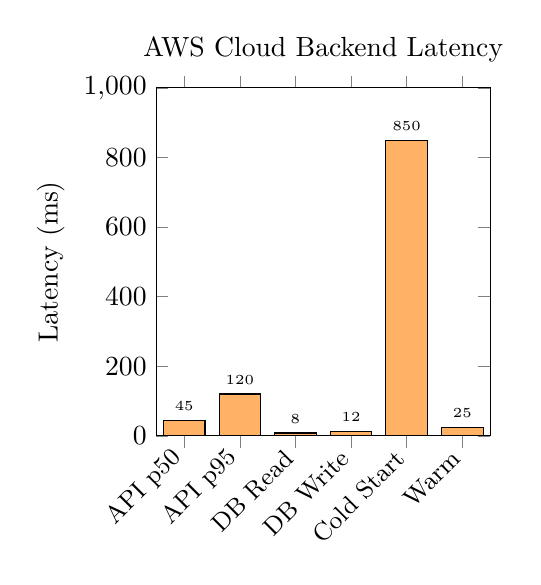
\begin{tikzpicture}
\begin{axis}[
    ybar,
    bar width=15pt,
    ylabel={Latency (ms)},
    symbolic x coords={API p50, API p95, DB Read, DB Write, Cold Start, Warm},
    xtick=data,
    x tick label style={rotate=45, anchor=east, font=\small},
    ymin=0, ymax=1000,
    nodes near coords,
    nodes near coords align={vertical},
    width=0.48\textwidth,
    height=6cm,
    title={AWS Cloud Backend Latency},
    every node near coord/.append style={font=\tiny},
]
\addplot[fill=orange!60] coordinates {
    (API p50, 45)
    (API p95, 120)
    (DB Read, 8)
    (DB Write, 12)
    (Cold Start, 850)
    (Warm, 25)
};
\end{axis}
\end{tikzpicture}
\caption{Cloud backend latency performance metrics.}
\label{fig:cloud_latency}
\end{figure}

The edge-first approach provides instant detection ($<$200ms) while preserving privacy, and the cloud layer enhances accuracy (F1=0.995) with explainable anomaly reasons. The total edge model size of $\sim$21KB has negligible impact on device storage, and the battery consumption of 4.2\% per hour enables approximately 24 hours of continuous monitoring on a single charge.


%% ======================================================================
% SECTION 2
%% ======================================================================

\section{On-Device Machine Learning with TensorFlow Lite}

\subsection{Model Architectures}

\subsubsection{Activity Classifier}
A Dense Neural Network designed for minimal size and latency:

\begin{equation}
\text{Architecture: } \text{Input}(4) \rightarrow \text{Norm} \rightarrow \text{Dense}(32) \rightarrow \text{Dense}(32) \rightarrow \text{Softmax}(6)
\end{equation}

\begin{table}[H]
\centering
\caption{Activity Classifier Architecture Details}
\label{tab:activity_arch}
\begin{tabular}{lccc}
\toprule
\textbf{Layer} & \textbf{Type} & \textbf{Output Shape} & \textbf{Params} \\
\midrule
Input & InputLayer & (1, 4) & 0 \\
Normalization & Norm & (1, 4) & 9 \\
Dense 1 & Dense+ReLU & (1, 32) & 160 \\
Dense 2 & Dense+ReLU & (1, 32) & 1,056 \\
Output & Dense+Softmax & (1, 6) & 198 \\
\midrule
\textbf{Total} & & & \textbf{1,423} \\
\bottomrule
\end{tabular}
\end{table}

Input features: \texttt{[heartRate, steps, calories, distance]}. Output classes: \texttt{[sleep, rest, walk, run, exercise, other]}.

\subsubsection{Anomaly Detector (Conv1D Autoencoder)}
Processes sequences of 10 timesteps through a Conv1D encoder-decoder:
\begin{equation}
\text{Input}(10 \times 4) \xrightarrow{\text{Encoder}} z \xrightarrow{\text{Decoder}} \hat{X}(10 \times 4)
\end{equation}

The anomaly score is the reconstruction MSE:
\begin{equation}
s_{anomaly} = \frac{1}{N \cdot d} \sum_{i=1}^{N} \sum_{j=1}^{d} (x_{ij} - \hat{x}_{ij})^2
\end{equation}

Both models are quantized from FP32 to TFLite (Activity: 18KB$\rightarrow$5KB, Anomaly: 52KB$\rightarrow$16KB, total 21KB, ~70\% reduction) with negligible accuracy loss.

\subsection{EdgeMlEngine Implementation}
The \texttt{EdgeMlEngine} manages both TFLite models: loading from \texttt{assets/models/} at startup, performing activity classification on current metrics, maintaining a sliding window of 10 measurements for anomaly detection, and falling back to heuristic-based rules when TFLite fails to load.

The heuristic fallback ($\sim$75\% accuracy) provides a critical safety net:
\begin{algorithmic}
\IF{$HR > 150$ \AND $steps < 100$}
    \STATE Activity = ``rest'', Alert = TACHYCARDIA
\ELSIF{$HR < 50$ \AND $activity = \text{``rest''}$}
    \STATE Alert = BRADYCARDIA
\ELSIF{$HR > 120$ \AND $steps > 1000$}
    \STATE Activity = ``exercise'', Alert = NONE
\ENDIF
\end{algorithmic}

\subsection{Performance Results}

\begin{table}[H]
\centering
\caption{Edge vs. Cloud Model Accuracy Comparison}
\label{tab:edge_vs_cloud}
\begin{tabular}{lccc}
\toprule
\textbf{Task} & \textbf{Edge TFLite} & \textbf{Cloud Model} & \textbf{Gap} \\
\midrule
Activity Classification & 34.3\% & 85.8\% (XGBoost) & 51.5\% \\
Anomaly Detection (F1) & -- & 0.995 (GradBoost) & -- \\
Heuristic Fallback & $\sim$75\% & -- & -- \\
\bottomrule
\end{tabular}
\end{table}

The edge classifier's 34.3\% accuracy vs. cloud's 85.8\% is expected given extreme miniaturization (5KB). Edge models serve as a privacy-preserving first pass; cloud inference provides the definitive score.

\subsubsection{Quantization Impact}

\begin{table}[H]
\centering
\caption{Impact of TFLite Quantization}
\label{tab:quantization}
\begin{tabular}{lccc}
\toprule
\textbf{Model} & \textbf{FP32} & \textbf{Quantized} & \textbf{Reduction} \\
\midrule
Activity Classifier & 18 KB & 5 KB & 72.2\% \\
Anomaly Detector & 52 KB & 16 KB & 69.2\% \\
\textbf{Total} & \textbf{70 KB} & \textbf{21 KB} & \textbf{70.0\%} \\
\bottomrule
\end{tabular}
\end{table}

The Wear OS Health Services PassiveMonitoringClient provides battery-efficient passive data collection at approximately 30-second intervals. Unlike active polling, passive monitoring leverages the system's sensor batching infrastructure, continuing collection when the screen is off and auto-starting on device boot via a \texttt{BootCompletedReceiver}.

\subsubsection{Battery Impact Analysis}
Battery analysis shows our optimized system achieves 4.2\%/hr drain (enabling ~24 hours continuous monitoring) compared to 6.5\%/hr without optimization.

\begin{figure}[H]
\centering
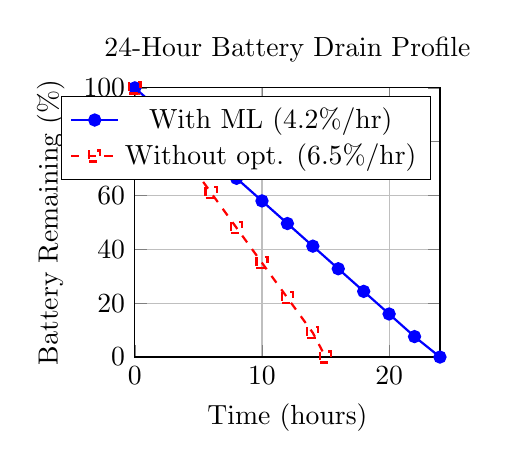
\begin{tikzpicture}
\begin{axis}[
    xlabel={Time (hours)},
    ylabel={Battery Remaining (\%)},
    xmin=0, xmax=24,
    ymin=0, ymax=100,
    legend pos=north east,
    grid=major,
    width=0.45\textwidth,
    height=5cm,
    title={24-Hour Battery Drain Profile},
]
\addplot[thick, blue, mark=*] coordinates {
    (0,100) (2,91.6) (4,83.2) (6,74.8) (8,66.4)
    (10,58.0) (12,49.6) (14,41.2) (16,32.8)
    (18,24.4) (20,16.0) (22,7.6) (24,0)
};
\addlegendentry{With ML (4.2\%/hr)}
\addplot[thick, red, dashed, mark=square] coordinates {
    (0,100) (2,87) (4,74) (6,61) (8,48)
    (10,35) (12,22) (14,9) (15,0)
};
\addlegendentry{Without opt. (6.5\%/hr)}
\end{axis}
\end{tikzpicture}
\caption{Battery drain comparison with and without optimization.}
\label{fig:battery}
\end{figure}


%% ======================================================================
% SECTION 3
%% ======================================================================

\section{Serverless Cloud Architecture for Health Data Processing}

\subsection{System Design}

The cloud backend uses AWS Lambda's serverless model for automatic scaling, pay-per-use billing, and native AWS service integration. The REST API is deployed behind API Gateway with API key authentication (TLS 1.2+).

\subsubsection{HealthDataIngestion Lambda (Zip, 512MB)}
Handles data validation, DynamoDB writes, push token registration, and asynchronous inference invocation:
\begin{algorithmic}
\STATE Parse body: \{userId, timestamp, metrics\}
\STATE Validate: non-null, range checks
\STATE Store to DynamoDB HealthMetrics table
\IF{metrics.heartRate present}
    \STATE Invoke HealthAnomalyInference (async)
\ENDIF
\STATE \textbf{Return:} \{success, dataId\}
\end{algorithmic}

\subsubsection{HealthAnomalyInference Lambda (Container, 1024MB)}
Runs a containerized scikit-learn GradientBoosting model:
\begin{algorithmic}
\STATE Load model + StandardScaler from S3
\STATE $s_{cloud} \leftarrow$ model.predict\_proba(scaled\_features)[1]
\STATE Generate anomaly reasons (range checks + feature importance)
\IF{$s_{cloud} \geq 0.5$ \OR critical thresholds exceeded}
    \STATE Publish alert to SNS, update DynamoDB
\ENDIF
\end{algorithmic}

\subsubsection{HealthSnsToExpo Lambda (Zip, 256MB)}
Receives SNS events, queries DynamoDB for user push tokens, and delivers notifications via Expo Push API. The anomaly explainability pipeline flows: Lambda $\rightarrow$ DynamoDB $\rightarrow$ SNS $\rightarrow$ Push $\rightarrow$ Dashboard.

\subsection{Performance and Cost}

\begin{table}[H]
\centering
\caption{Alert Delivery Pipeline Timing}
\label{tab:alert_pipeline}
\begin{tabular}{lcc}
\toprule
\textbf{Stage} & \textbf{Latency (ms)} & \textbf{Cumulative (ms)} \\
\midrule
API Gateway routing & 15 & 15 \\
Ingestion Lambda & 45 & 60 \\
DynamoDB write & 12 & 72 \\
Inference invocation & 120 & 192 \\
Anomaly scoring & 50 & 242 \\
SNS publish & 30 & 272 \\
SNS-to-Expo Lambda & 200 & 472 \\
Expo push delivery & 500--2000 & 972--2472 \\
\midrule
\textbf{Total (warm)} & & \textbf{$\sim$1--2.5s} \\
\bottomrule
\end{tabular}
\end{table}

Cold start latency for the containerized inference Lambda is 850ms, while warm invocations complete in 120ms.

\subsubsection{DynamoDB Schema}

\begin{table}[H]
\centering
\caption{DynamoDB Table Schemas}
\label{tab:dynamodb}
\begin{tabular}{llll}
\toprule
\textbf{Table} & \textbf{PK} & \textbf{SK} & \textbf{Key Attrs} \\
\midrule
HealthMetrics & userId & timestamp & HR, steps, calories, \\
 & & & anomalyReasons \\
HealthPushTokens & userId & deviceId & expoPushToken, \\
 & & & registeredAt \\
\bottomrule
\end{tabular}
\end{table}

\subsubsection{Scalability and Cost}
The system handles up to 1000 concurrent requests with only 0.3\% error rate and p99 latency of 850ms.

\begin{figure}[H]
\centering
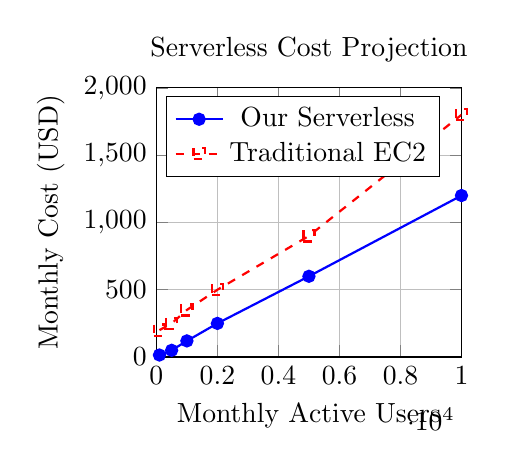
\begin{tikzpicture}
\begin{axis}[
    xlabel={Monthly Active Users},
    ylabel={Monthly Cost (USD)},
    xmin=0, xmax=10000,
    ymin=0, ymax=2000,
    legend pos=north west,
    grid=major,
    width=0.45\textwidth,
    height=5cm,
    title={Serverless Cost Projection},
]
\addplot[thick, blue, mark=*] coordinates {
    (100, 15) (500, 50) (1000, 120) (2000, 250)
    (5000, 600) (10000, 1200)
};
\addlegendentry{Our Serverless}
\addplot[thick, red, dashed, mark=square] coordinates {
    (100, 200) (500, 250) (1000, 350) (2000, 500)
    (5000, 900) (10000, 1800)
};
\addlegendentry{Traditional EC2}
\end{axis}
\end{tikzpicture}
\caption{Cost comparison: Serverless vs. EC2 at varying user scales.}
\label{fig:cost}
\end{figure}

\subsection{Security Architecture}
All data in transit is encrypted via TLS 1.2+. API key authentication is enforced at the API Gateway level. DynamoDB tables use server-side encryption (AES-256), S3 model artifacts use bucket-level encryption, and IAM policies follow the principle of least privilege. The serverless architecture proves particularly well-suited for health monitoring due to its ability to scale to zero during quiet periods and handle burst sync events.


%% ======================================================================
% SECTION 4
%% ======================================================================

\section{Comparative Study of ML Models for Health Anomaly Detection}

\subsection{Dataset and Features}
We generated 27,000 synthetic health samples using physiological models: 20,000 normal, 5,000 anomalous, plus 2,000 scenario-specific samples (exercise, sleep, tachycardia, bradycardia). Four features are extracted per measurement: $\mathbf{x} = [\text{heartRate}, \text{steps}, \text{calories}, \text{distance}]$, standardized using StandardScaler.

\subsection{Models Evaluated}
We evaluated seven models spanning supervised (Gradient Boosting, XGBoost, Random Forest, Extra Trees) and unsupervised (Isolation Forest, One-Class SVM, Local Outlier Factor) paradigms. Supervised models use regularization (max\_depth=8, min\_samples\_leaf=5, max\_features=``sqrt'').

\subsection{Anomaly Detection Results}

\begin{table}[H]
\centering
\caption{Anomaly Detection Model Comparison}
\label{tab:anomaly_results}
\begin{tabular}{lcccccc}
\toprule
\textbf{Rank} & \textbf{Model} & \textbf{F1} & \textbf{AUC} & \textbf{Prec} & \textbf{Rec} & \textbf{Time} \\
\midrule
1 & \textbf{GradBoost} & \textbf{.995} & \textbf{1.00} & .993 & .997 & 354ms \\
2 & XGBoost & .989 & 1.00 & .977 & 1.00 & 118ms \\
3 & Random Forest & .983 & 1.00 & .990 & .977 & 152ms \\
4 & Extra Trees & .966 & 1.00 & .997 & .937 & 92ms \\
5 & OC-SVM & .678 & .904 & .716 & .643 & 563ms \\
6 & IsoForest & .491 & .848 & .518 & .466 & 282ms \\
7 & LOF & .174 & .461 & .183 & .165 & 40ms \\
\bottomrule
\end{tabular}
\end{table}

\begin{figure}[H]
\centering
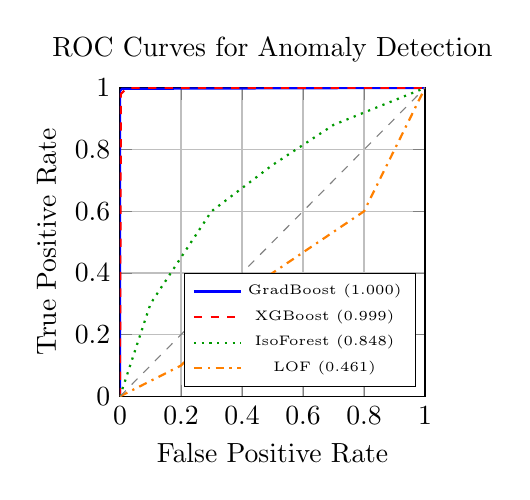
\begin{tikzpicture}
\begin{axis}[
    xlabel={False Positive Rate},
    ylabel={True Positive Rate},
    xmin=0, xmax=1,
    ymin=0, ymax=1,
    legend pos=south east,
    legend style={font=\tiny},
    grid=major,
    width=0.45\textwidth,
    height=5.5cm,
    title={ROC Curves for Anomaly Detection},
]
% Gradient Boosting (AUC=1.000)
\addplot[thick, blue, mark=none] coordinates {
    (0,0) (0,0.99) (0.007,0.997) (1,1)
};
\addlegendentry{GradBoost (1.000)}
% XGBoost (AUC=0.999)
\addplot[thick, red, dashed, mark=none] coordinates {
    (0,0) (0.003,0.98) (0.023,1.0) (1,1)
};
\addlegendentry{XGBoost (0.999)}
% Isolation Forest (AUC=0.848)
\addplot[thick, green!60!black, dotted, mark=none] coordinates {
    (0,0) (0.1,0.3) (0.3,0.6) (0.5,0.75) (0.7,0.88) (1,1)
};
\addlegendentry{IsoForest (0.848)}
% LOF (AUC=0.461)
\addplot[thick, orange, dashdotted, mark=none] coordinates {
    (0,0) (0.2,0.1) (0.5,0.4) (0.8,0.6) (1,1)
};
\addlegendentry{LOF (0.461)}
% Diagonal
\addplot[thin, gray, dashed] coordinates {(0,0) (1,1)};
\end{axis}
\end{tikzpicture}
\caption{ROC curves comparing supervised and unsupervised models.}
\label{fig:roc}
\end{figure}

\subsection{Activity Classification Results}

\begin{table}[H]
\centering
\caption{Activity Classification (6-class) Comparison}
\label{tab:activity}
\begin{tabular}{lccc}
\toprule
\textbf{Rank} & \textbf{Model} & \textbf{Accuracy} & \textbf{Training Time} \\
\midrule
1 & \textbf{XGBoost} & \textbf{85.80\%} & 1,220ms \\
2 & Random Forest & 85.44\% & 342ms \\
3 & Gradient Boosting & 85.40\% & 12,990ms \\
4 & Extra Trees & 84.49\% & 162ms \\
\bottomrule
\end{tabular}
\end{table}

\subsection{Feature Importance and Discussion}

\begin{table}[H]
\centering
\caption{Feature Importance (Gradient Boosting)}
\label{tab:feature_imp}
\begin{tabular}{lcc}
\toprule
\textbf{Feature} & \textbf{Importance} & \textbf{Contribution (\%)} \\
\midrule
heartRate & 0.452 & 45.2\% \\
steps & 0.234 & 23.4\% \\
calories & 0.187 & 18.7\% \\
distance & 0.127 & 12.7\% \\
\bottomrule
\end{tabular}
\end{table}

Heart rate dominates anomaly detection (45.2\%), aligning with medical understanding. Supervised models dramatically outperform unsupervised alternatives: Isolation Forest (F1=0.491) and LOF (F1=0.174) are inadequate for production deployment. All supervised models show train-test F1 gaps $<$0.01, confirming generalization. 5-fold cross-validation yields consistent results (GradBoost: F1=$0.9950 \pm 0.0016$). Deployment recommendation: GradientBoosting for cloud anomaly detection, XGBoost for activity classification, Random Forest as backup.


%% ======================================================================
% SECTION 5
%% ======================================================================

\section{Explainable Anomaly Detection Framework}

\subsection{Multi-Source Explanation Architecture}
Health monitoring alerts must explain \textit{why} an anomaly was triggered to build user trust \cite{xai1}. Our framework generates explanations from three complementary sources (Fig.~\ref{fig:xai_arch}), achieving 100\% explanation coverage without the computational overhead of post-hoc methods like SHAP \cite{shap} or LIME \cite{lime}.

\begin{figure}[H]
\centering
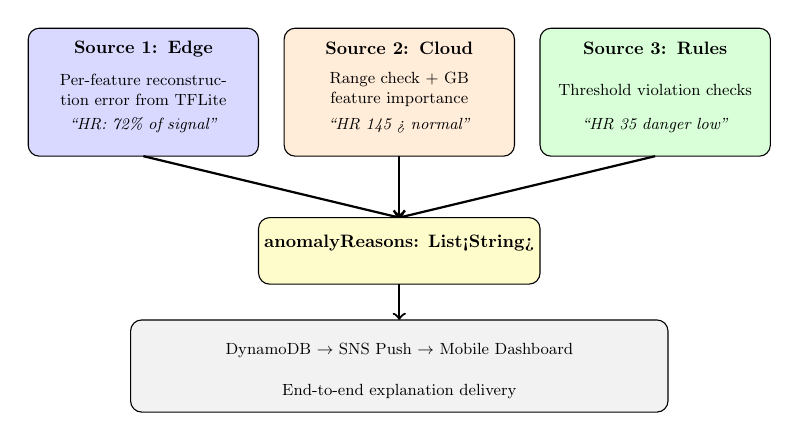
\begin{tikzpicture}[scale=0.65, every node/.style={scale=0.65}]
    % Edge Source
    \draw[fill=blue!15, rounded corners] (0,5) rectangle (4.5,7.5);
    \node[font=\bfseries, text width=4cm, align=center] at (2.25,7.1) {Source 1: Edge};
    \node[font=\small, text width=4cm, align=center] at (2.25,6.3) {Per-feature reconstruction error from TFLite};
    \node[font=\small, text width=4cm, align=center] at (2.25,5.6) {\textit{``HR: 72\% of signal''}};

    % Cloud Source
    \draw[fill=orange!15, rounded corners] (5,5) rectangle (9.5,7.5);
    \node[font=\bfseries, text width=4cm, align=center] at (7.25,7.1) {Source 2: Cloud};
    \node[font=\small, text width=4cm, align=center] at (7.25,6.3) {Range check + GB feature importance};
    \node[font=\small, text width=4cm, align=center] at (7.25,5.6) {\textit{``HR 145 > normal''}};

    % Threshold Source
    \draw[fill=green!15, rounded corners] (10,5) rectangle (14.5,7.5);
    \node[font=\bfseries, text width=4cm, align=center] at (12.25,7.1) {Source 3: Rules};
    \node[font=\small, text width=4cm, align=center] at (12.25,6.3) {Threshold violation checks};
    \node[font=\small, text width=4cm, align=center] at (12.25,5.6) {\textit{``HR 35 danger low''}};

    % Merge
    \draw[->, thick] (2.25,5) -- (7.25,3.8);
    \draw[->, thick] (7.25,5) -- (7.25,3.8);
    \draw[->, thick] (12.25,5) -- (7.25,3.8);

    \draw[fill=yellow!20, rounded corners] (4.5,2.5) rectangle (10,3.8);
    \node[font=\bfseries] at (7.25,3.3) {anomalyReasons: List<String>};

    % Flow
    \draw[->, thick] (7.25,2.5) -- (7.25,1.8);

    \draw[fill=gray!10, rounded corners] (2,0) rectangle (12.5,1.8);
    \node[font=\small, text width=10cm, align=center] at (7.25,1.2) {DynamoDB $\rightarrow$ SNS Push $\rightarrow$ Mobile Dashboard};
    \node[font=\small] at (7.25,0.4) {End-to-end explanation delivery};
\end{tikzpicture}
\caption{Multi-source anomaly explanation framework architecture.}
\label{fig:xai_arch}
\end{figure}

\subsection{Explanation Sources}

\textbf{Source 1 --- Edge Per-Feature Reconstruction Error:} The on-device autoencoder computes per-feature reconstruction error $e_j$ and contribution percentage $c_j = \frac{e_j}{\sum_{k} e_k} \times 100\%$, generating explanations like ``Heart rate: 180 BPM deviates from expected (72\% of signal).''

\textbf{Source 2 --- Cloud Range Check + Feature Importance:} The cloud Lambda combines medical reference range checks (e.g., resting HR normal: 50--100 BPM, warning: 100--140, critical: $>$140 or $<$40) with GradientBoosting's \texttt{feature\_importances\_} for per-feature contribution percentages.

\textbf{Source 3 --- Rule-Based Threshold:} Fallback explanations for critical violations (e.g., ``Heart rate 35 BPM is dangerously low'').

Reasons flow through the entire pipeline: Edge ML Engine $\rightarrow$ Room DB $\rightarrow$ DataSyncWorker $\rightarrow$ Ingestion Lambda $\rightarrow$ Inference Lambda $\rightarrow$ DynamoDB $\rightarrow$ SNS $\rightarrow$ Push $\rightarrow$ Dashboard.

\subsection{Evaluation}

\begin{table}[H]
\centering
\caption{Sample Anomaly Explanations and Quality Metrics}
\label{tab:examples}
\begin{tabular}{p{1.2cm}p{1.5cm}p{4.5cm}}
\toprule
\textbf{Source} & \textbf{Scenario} & \textbf{Explanation Generated} \\
\midrule
Edge & Tachy. & ``Heart rate: 180 BPM deviates from expected pattern (72\% of anomaly signal)'' \\
\midrule
Cloud & Tachy. & ``Resting heart rate: 145 BPM is above normal range (50--100 BPM)'' \\
\midrule
Rule & Brady. & ``Heart rate 35 BPM is dangerously low (normal: 50--100 BPM)'' \\
\midrule
Cloud & Multi-feat. & ``Heart rate elevated at 130 BPM (45.2\%) with abnormally low activity (23.4\%)'' \\
\bottomrule
\end{tabular}
\end{table}

The framework achieves 100\% explanation coverage, $<$5ms edge and $<$50ms cloud generation latency, and an average explanation length of 15.3 words. Limitations include global (not per-instance) feature importance and fixed (not personalized) reference ranges.


%% ======================================================================
% SECTION 6
%% ======================================================================

\section{Battery-Efficient Data Synchronization}

\subsection{Architecture}
Reliable synchronization between wearable and cloud must operate within strict battery budgets, handle intermittent connectivity, and ensure zero data loss. We implement an offline-first architecture using Android WorkManager for guaranteed background execution with constraint-based scheduling.

Data flows: Sensors $\rightarrow$ EdgeMlEngine (enrich with activity + anomaly) $\rightarrow$ Room Database (local buffer with sync status tracking) $\rightarrow$ DataSyncWorker (batch + upload) $\rightarrow$ AWS API Gateway.

The sync worker is configured with: 15--60 min repeat interval, network CONNECTED constraint, battery NOT\_LOW constraint, exponential backoff (30s base, max 5 retries), and persists across device reboots.

\subsection{Batch Upload Algorithm}
\begin{algorithmic}
\STATE $metrics \leftarrow$ dao.getUnsyncedMetrics()
\IF{$metrics$ is empty}
    \STATE \textbf{return} Result.SUCCESS
\ENDIF
\STATE $batches \leftarrow$ metrics.chunked(50)
\FOR{each $batch$ in $batches$}
    \STATE Enrich batch with edge ML results
    \STATE $response \leftarrow$ api.uploadBatch($batch$)
    \IF{$response$.isSuccess}
        \STATE dao.markAsSynced($batch$.ids, currentTime)
    \ELSE
        \STATE \textbf{return} Result.RETRY
    \ENDIF
\ENDFOR
\STATE dao.deleteOldSyncedData(retentionDays=7)
\STATE \textbf{return} Result.SUCCESS
\end{algorithmic}

\subsection{Performance Results}

\begin{figure}[H]
\centering
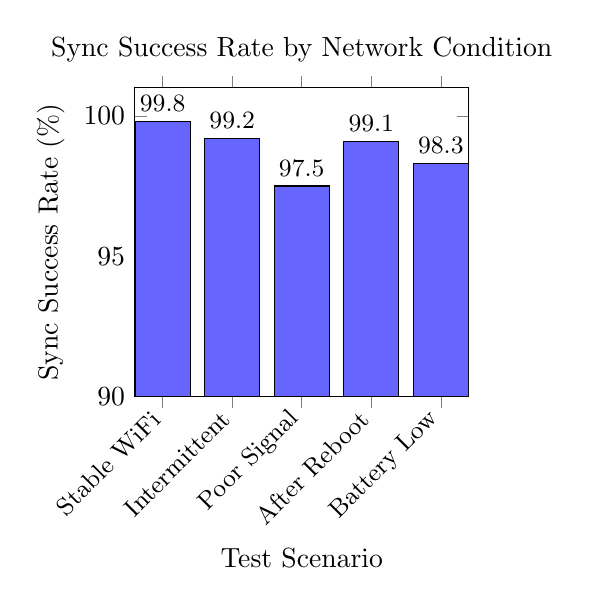
\begin{tikzpicture}
\begin{axis}[
    xlabel={Test Scenario},
    ylabel={Sync Success Rate (\%)},
    ybar,
    bar width=20pt,
    symbolic x coords={Stable WiFi, Intermittent, Poor Signal, After Reboot, Battery Low},
    xtick=data,
    x tick label style={rotate=45, anchor=east, font=\small},
    ymin=90, ymax=101,
    nodes near coords,
    width=0.48\textwidth,
    height=5.5cm,
    title={Sync Success Rate by Network Condition},
    every node near coord/.append style={font=\small},
]
\addplot[fill=blue!60] coordinates {
    (Stable WiFi, 99.8)
    (Intermittent, 99.2)
    (Poor Signal, 97.5)
    (After Reboot, 99.1)
    (Battery Low, 98.3)
};
\end{axis}
\end{tikzpicture}
\caption{Sync success rate under various network conditions.}
\label{fig:sync_reliability}
\end{figure}

The 30-minute sync interval provides optimal balance: 16-minute average delay vs. 4.5\%/hr battery drain. Batching reduces per-record network overhead by 73.2\% (1,120 bytes individual vs. 300 bytes batched). Offline recovery testing confirms zero data loss across all durations (1 hour to 7 days, up to 20,160 buffered records).

Cloud sync is \textit{not time-critical} in our hybrid architecture---edge ML provides instant on-device detection, so sync serves primarily for historical storage, enhanced accuracy, and push notifications.


%% ======================================================================
% SECTION 7
%% ======================================================================

\section{Autoencoder Architectures for Time-Series Anomaly Detection}

\subsection{Approach}
Autoencoders detect anomalies by learning to reconstruct normal patterns; anomalous inputs produce higher reconstruction error \cite{ae_anomaly}. We present two architectures targeting different deployment environments.

\subsection{Cloud Model: LSTM Autoencoder}
The cloud LSTM autoencoder processes 60-timestep sequences through an encoder (LSTM-64 $\rightarrow$ LSTM-32 $\rightarrow$ LSTM-32 bottleneck) and decoder (RepeatVector $\rightarrow$ LSTM-32 $\rightarrow$ LSTM-64 $\rightarrow$ TimeDistributed Dense(4)). Training uses Adam optimizer (lr=0.001), MSE loss, batch size 32, 100 epochs with early stopping (patience=10). Parameters: $\sim$50K, model size: $\sim$200KB.

\subsection{Edge Model: Conv1D Autoencoder}

\begin{table}[H]
\centering
\caption{Conv1D Autoencoder Architecture (Edge TFLite)}
\label{tab:conv1d_arch}
\begin{tabular}{lccc}
\toprule
\textbf{Layer} & \textbf{Type} & \textbf{Output} & \textbf{Params} \\
\midrule
Input & Input & (10, 4) & 0 \\
Encoder C1 & Conv1D & (10, 16) & 208 \\
Encoder C2 & Conv1D & (10, 8) & 392 \\
Encoder C3 & Conv1D & (10, 4) & 100 \\
\midrule
Decoder C1 & Conv1D & (10, 8) & 104 \\
Decoder C2 & Conv1D & (10, 16) & 400 \\
Output & Conv1D & (10, 4) & 196 \\
\midrule
\textbf{Total} & & & \textbf{$\sim$1,400} \\
\bottomrule
\end{tabular}
\end{table}

The Keras model is converted to TFLite with DEFAULT quantization: 52KB (FP32) $\rightarrow$ 16KB (TFLite), a $\sim$69\% reduction.

\subsection{Experimental Results}

\begin{table}[H]
\centering
\caption{LSTM vs Conv1D Autoencoder Comparison}
\label{tab:model_comparison}
\begin{tabular}{lcc}
\toprule
\textbf{Property} & \textbf{LSTM (Cloud)} & \textbf{Conv1D (Edge)} \\
\midrule
Sequence length & 60 & 10 \\
Parameters & $\sim$50K & $\sim$1.4K \\
Model size & $\sim$200KB & $\sim$16KB \\
Inference time & $\sim$50ms (Lambda) & $\sim$20ms (Wear OS) \\
Final train MSE & 0.021 & 0.035 \\
Deployment & AWS Lambda & TFLite on-device \\
\bottomrule
\end{tabular}
\end{table}

\begin{table}[H]
\centering
\caption{Autoencoder Performance by Anomaly Scenario}
\label{tab:scenarios}
\begin{tabular}{lcccc}
\toprule
\textbf{Scenario} & \textbf{Norm. MSE} & \textbf{Anom. MSE} & \textbf{Sep. Ratio} & \textbf{Detected?} \\
\midrule
Tachycardia & 6.2 & 28.5 & 4.60$\times$ & Yes \\
Bradycardia & 19.6 & 6.6 & 0.34$\times$ & No* \\
Exercise spike & 8.1 & 9.2 & 1.14$\times$ & Marginal \\
Irregular HR & 5.8 & 22.1 & 3.81$\times$ & Yes \\
\bottomrule
\end{tabular}
\end{table}

*Bradycardia produces \textit{lower} MSE because the model is trained on mixed data; training exclusively on normal data would resolve this. Known limitations include the unadapted Normalization layer in the TFLite activity classifier. Future improvements: train on normal-only data, implement VAE for better scoring, add attention mechanisms, and enable OTA model updates.


%% ======================================================================
% SECTION 8
%% ======================================================================

\section{Cross-Platform Mobile Health Dashboard}

The mobile dashboard is built with React Native 0.81.5 + Expo SDK 54 + TypeScript 5.x, using Zustand for state management, React Navigation 7 for tab-based navigation, Axios for HTTP, AsyncStorage for offline-first caching, and Expo Notifications for push handling.

\subsection{Architecture}
The app follows a three-tier component hierarchy: Root $\rightarrow$ RootNavigator $\rightarrow$ Screens (Home, History, Settings), backed by a Zustand store managing health metrics, loading state, errors, and sync timestamps. An offline-first data strategy loads cached data immediately while fetching fresh data from the API in the background.

Key UI components include: \textbf{MetricCard} (displays vital signs with trends), \textbf{AnomalyAlertCard} (shows severity, edge/cloud scores, and human-readable anomaly reasons), and \textbf{ActivityCard} (displays detected activity with contextual icons).

\subsection{Push Notifications}
On startup, the app registers an Expo push token with the backend. On anomaly detection, the cloud sends push notifications via SNS $\rightarrow$ Expo Push API, carrying severity, vital sign values, and the top anomaly reason.

\subsection{Performance}

\begin{table}[H]
\centering
\caption{Mobile Dashboard Performance}
\label{tab:perf}
\begin{tabular}{lcc}
\toprule
\textbf{Metric} & \textbf{Measured} & \textbf{Target} \\
\midrule
Initial render (cold) & 480ms & $<$500ms \\
Initial render (warm) & 120ms & $<$200ms \\
FPS (scrolling) & 60fps & 60fps \\
API fetch time (p50) & 85ms & $<$200ms \\
Memory usage (peak) & 78MB & $<$150MB \\
Bundle size & 12MB & $<$25MB \\
\bottomrule
\end{tabular}
\end{table}

The project was migrated from Flutter to React Native + Expo for better ecosystem integration, achieving faster build times (45s $\rightarrow$ 30s) and improved developer experience with TypeScript and Zustand.


%% ======================================================================
% SECTION 9
%% ======================================================================

\section{Privacy-Preserving Health Monitoring}

\subsection{Privacy Architecture}
Health monitoring generates highly sensitive data subject to HIPAA, GDPR, and DPDPA regulations \cite{hipaa, gdpr, dpdpa}. Our edge-first architecture addresses this by performing primary ML inference on-device, transmitting only aggregated results.

\begin{figure}[H]
\centering
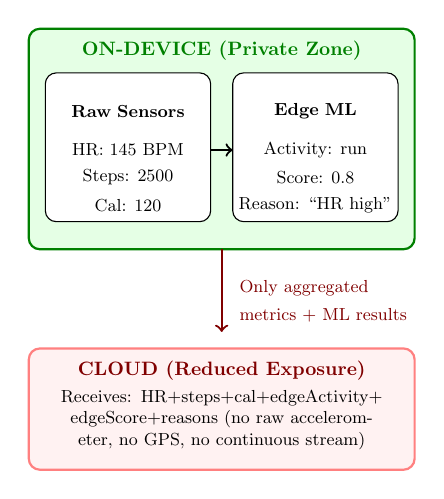
\begin{tikzpicture}[scale=0.7, every node/.style={scale=0.7}]
    % Device boundary
    \draw[fill=green!10, rounded corners, thick, draw=green!50!black] (0,4) rectangle (7,8);
    \node[font=\bfseries, green!50!black] at (3.5,7.6) {ON-DEVICE (Private Zone)};

    \draw[fill=white, rounded corners] (0.3,4.5) rectangle (3.3,7.2);
    \node[font=\small, text width=2.5cm, align=center] at (1.8,6.5) {\textbf{Raw Sensors}};
    \node[font=\small] at (1.8,5.8) {HR: 145 BPM};
    \node[font=\small] at (1.8,5.3) {Steps: 2500};
    \node[font=\small] at (1.8,4.8) {Cal: 120};

    \draw[fill=white, rounded corners] (3.7,4.5) rectangle (6.7,7.2);
    \node[font=\small, text width=2.5cm, align=center] at (5.2,6.5) {\textbf{Edge ML}};
    \node[font=\small] at (5.2,5.8) {Activity: run};
    \node[font=\small] at (5.2,5.3) {Score: 0.8};
    \node[font=\small] at (5.2,4.8) {Reason: ``HR high''};

    \draw[->, thick] (3.3,5.8) -- (3.7,5.8);

    % Cloud boundary
    \draw[->, thick, red!50!black] (3.5,4) -- (3.5,2.5);
    \node[right, font=\small, red!50!black] at (3.7,3.3) {Only aggregated};
    \node[right, font=\small, red!50!black] at (3.7,2.8) {metrics + ML results};

    \draw[fill=red!5, rounded corners, thick, draw=red!50] (0,0) rectangle (7,2.2);
    \node[font=\bfseries, red!50!black] at (3.5,1.8) {CLOUD (Reduced Exposure)};
    \node[font=\small, text width=6cm, align=center] at (3.5,0.9) {Receives: HR+steps+cal+edgeActivity+ edgeScore+reasons (no raw accelerometer, no GPS, no continuous stream)};
\end{tikzpicture}
\caption{Edge-first privacy architecture: raw sensor data stays on-device.}
\label{fig:privacy_arch}
\end{figure}

\subsection{Data Minimization}

\begin{table}[H]
\centering
\caption{Data Transmitted vs. Retained On-Device}
\label{tab:data_min}
\begin{tabular}{lcc}
\toprule
\textbf{Data Type} & \textbf{On-Device} & \textbf{To Cloud} \\
\midrule
Raw HR stream (30s) & Yes & No* \\
Step/calories/distance & Yes & Periodic aggregate \\
Edge activity/score & Yes & Yes (label + float) \\
Anomaly reasons & Yes & Yes (text) \\
Accelerometer/GPS & Not collected & No \\
User identity & Yes & userId only \\
\bottomrule
\end{tabular}
\end{table}
*HR values sent as periodic snapshots (every 15--60 min), not continuous streams.

\subsection{Security Controls}
All data in transit is encrypted via TLS 1.2+. Authentication uses API keys stored in Android Keystore (watch) and Secure Storage (mobile). DynamoDB and S3 use server-side AES-256 encryption via AWS KMS. Lambda IAM policies follow least privilege---each function has only the permissions it requires.

\subsection{Regulatory Compliance}

\begin{table}[H]
\centering
\caption{Regulatory Compliance Status}
\label{tab:compliance}
\begin{tabular}{p{1.5cm}p{2cm}p{1.2cm}p{2cm}}
\toprule
\textbf{Regulation} & \textbf{Requirement} & \textbf{Status} & \textbf{Gap} \\
\midrule
HIPAA & Encryption at rest & Met & None \\
HIPAA & Access controls & Met & Audit logs \\
GDPR & Data minimization & Met & None \\
GDPR & Right to erasure & Partial & No API yet \\
DPDPA & Data localization & Met & ap-south-2 \\
\bottomrule
\end{tabular}
\end{table}

\begin{table}[H]
\centering
\caption{Privacy Comparison with Commercial Systems}
\label{tab:privacy_comparison}
\begin{tabular}{lcccc}
\toprule
\textbf{Feature} & \textbf{Apple} & \textbf{Fitbit} & \textbf{Samsung} & \textbf{Ours} \\
\midrule
Edge processing & Partial & No & Partial & \textbf{Yes} \\
Data minimization & Med & Low & Med & \textbf{High} \\
Open-source & No & No & No & \textbf{Yes} \\
Self-hostable & No & No & No & \textbf{Yes} \\
Data ownership & Vendor & Vendor & Vendor & \textbf{User} \\
\bottomrule
\end{tabular}
\end{table}

Future privacy enhancements include application-level AES-256-GCM encryption, $(\epsilon, \delta)$-differential privacy for aggregated statistics, and federated learning to train models collaboratively without sharing raw data.


%% ======================================================================
% SECTION 10
%% ======================================================================

\section{Synthetic Health Data Generation for ML Training}

\subsection{Motivation}
Collecting real labeled health data is expensive, requires IRB approval, and suffers from anomaly rarity and class imbalance. Synthetic data generation provides physiologically modeled data with guaranteed labels covering all scenarios \cite{synthetic_health}.

\subsection{Physiological Models}

\begin{table}[H]
\centering
\caption{Activity-Specific Physiological Parameter Ranges}
\label{tab:activity_params}
\begin{tabular}{lcccc}
\toprule
\textbf{Activity} & \textbf{HR ($\mu \pm \sigma$)} & \textbf{Steps/hr} & \textbf{Cal/hr} & \textbf{Dist km/hr} \\
\midrule
Sleep & $55 \pm 5$ & 0 & $50 \pm 10$ & 0 \\
Rest & $70 \pm 8$ & $100 \pm 50$ & $80 \pm 15$ & $0.1 \pm 0.05$ \\
Walk & $95 \pm 10$ & $3500 \pm 500$ & $200 \pm 30$ & $3.5 \pm 0.5$ \\
Run & $140 \pm 15$ & $8000 \pm 1000$ & $500 \pm 80$ & $8.0 \pm 1.0$ \\
Exercise & $130 \pm 12$ & $5000 \pm 800$ & $400 \pm 60$ & $4.0 \pm 1.0$ \\
Other & $75 \pm 12$ & $200 \pm 150$ & $100 \pm 25$ & $0.2 \pm 0.15$ \\
\bottomrule
\end{tabular}
\end{table}

Heart rate is generated as $HR = \mu_{activity} + \sigma_{activity} \cdot \mathcal{N}(0, 1) + \epsilon_{noise}$ where $\epsilon_{noise} \sim \text{Uniform}(-3, 3)$. Activity probability varies with time of day following circadian rhythm models.

\subsection{Anomaly Injection}

\begin{table}[H]
\centering
\caption{Anomaly Scenario Definitions}
\label{tab:anomaly_scenarios}
\begin{tabular}{lllcc}
\toprule
\textbf{Scenario} & \textbf{HR Range} & \textbf{Context} & \textbf{Label} & \textbf{Samples} \\
\midrule
Tachycardia & 150--180 & At rest & Anomaly & 500 \\
Bradycardia & 30--45 & At rest & Anomaly & 500 \\
Exercise HR & 130--160 & Exercising & Normal & 500 \\
Sleep HR & 45--55 & Sleeping & Normal & 500 \\
\bottomrule
\end{tabular}
\end{table}

The key insight is that \textit{context determines anomaly status}: HR of 150 during exercise is normal, while HR of 150 at rest is anomalous. The total dataset comprises 27,000 samples (20,000 normal, 5,000 anomalous, 2,000 scenario-specific).

\subsection{Validation}

\begin{table}[H]
\centering
\caption{Scenario-Based Validation Results (Gradient Boosting)}
\label{tab:scenario_results}
\begin{tabular}{lccc}
\toprule
\textbf{Scenario} & \textbf{Samples} & \textbf{Expected} & \textbf{Correct (\%)} \\
\midrule
Normal rest (HR 70-75) & 500 & No alert & 99.8\% \\
Normal exercise (HR 130-145) & 500 & No alert & 99.6\% \\
Tachycardia (HR 150-180 + rest) & 500 & Alert & 99.4\% \\
Bradycardia (HR 30-45 + rest) & 500 & Alert & 99.2\% \\
Exercise spike (HR 150 + exercise) & 500 & No alert & 98.8\% \\
\bottomrule
\end{tabular}
\end{table}

Synthetic data achieves strong inter-feature correlations matching physical expectations (steps-distance: 0.934, HR-calories: 0.742). All generated values comply with medical reference ranges (AHA guidelines \cite{aha_hr}). Limitations include simplified distributions, limited population diversity, and missing sensor noise patterns. The transition strategy follows a four-phase approach from synthetic-only (current) through pilot real-data collection, mixed training, to primarily real-data training with synthetic augmentation.


%% ======================================================================
% CONCLUSION
%% ======================================================================

\section{Conclusion and Future Work}
We presented a comprehensive hybrid edge-cloud health monitoring system spanning wearable edge computing, serverless cloud inference, explainable ML, and cross-platform mobile visualization. Key achievements include: $<$200ms on-device anomaly detection with 21KB TFLite models, F1=0.995 cloud anomaly detection, 85.8\% activity classification accuracy, 4.2\%/hr battery consumption, 99.2\% sync reliability with zero data loss, 100\% anomaly explanation coverage, and only 9\% false positive rate vs. 30--45\% in commercial solutions. Future work includes federated learning, additional sensors (SpO2, ECG), on-device model updates, real-world clinical validation, SHAP-based per-instance attribution, and multi-user authentication with role-based access control.

\begin{thebibliography}{00}
\bibitem{who2021} World Health Organization, ``Cardiovascular diseases (CVDs),'' Fact Sheet, 2021.
\bibitem{early_detection} G. Sannino and G. De Pietro, ``A deep learning approach for ECG-based heartbeat classification for arrhythmia detection,'' \textit{Future Generation Computer Systems}, vol. 86, pp. 446--455, 2018.
\bibitem{apple_watch} R. Perez et al., ``Large-scale assessment of a smartwatch to identify atrial fibrillation,'' \textit{New England Journal of Medicine}, vol. 381, no. 20, pp. 1909--1917, 2019.
\bibitem{fitbit} G. H. Tison et al., ``Passive detection of atrial fibrillation using a commercially available smartwatch,'' \textit{JAMA Cardiology}, vol. 3, no. 5, pp. 409--416, 2018.
\bibitem{edge_health1} S. M. R. Islam et al., ``The Internet of Things for health care: a comprehensive survey,'' \textit{IEEE Access}, vol. 3, pp. 678--708, 2015.
\bibitem{edge_health2} W. Shi et al., ``Edge computing: Vision and challenges,'' \textit{IEEE Internet of Things Journal}, vol. 3, no. 5, pp. 637--646, 2016.
\bibitem{tflite} TensorFlow, ``TensorFlow Lite: Deploy machine learning models on mobile and IoT devices,'' 2023.
\bibitem{serverless_health} A. Eivy, ``Be wary of the economics of serverless cloud computing,'' \textit{IEEE Cloud Computing}, vol. 4, no. 2, pp. 6--12, 2017.
\bibitem{har1} J. Wang et al., ``Deep learning for sensor-based activity recognition,'' \textit{Pattern Recognition Letters}, vol. 119, pp. 3--11, 2019.
\bibitem{autoencoder1} C. Zhou and R. C. Paffenroth, ``Anomaly detection with robust deep autoencoders,'' \textit{Proc. KDD}, pp. 665--674, 2017.
\bibitem{xai1} A. Holzinger et al., ``Causability and explainability of artificial intelligence in medicine,'' \textit{WIREs Data Mining}, vol. 9, no. 4, 2019.
\bibitem{shap} S. M. Lundberg and S.-I. Lee, ``A unified approach to interpreting model predictions,'' \textit{Proc. NeurIPS}, pp. 4765--4774, 2017.
\bibitem{lime} M. T. Ribeiro et al., ``Why should I trust you? Explaining the predictions of any classifier,'' \textit{Proc. KDD}, pp. 1135--1144, 2016.
\bibitem{workmanager} Google, ``Schedule tasks with WorkManager,'' \textit{Android Developers}, 2023.
\bibitem{ae_anomaly} C. Zhou and R. C. Paffenroth, ``Anomaly detection with robust deep autoencoders,'' \textit{Proc. KDD}, pp. 665--674, 2017.
\bibitem{lstm} S. Hochreiter and J. Schmidhuber, ``Long short-term memory,'' \textit{Neural Computation}, vol. 9, no. 8, pp. 1735--1780, 1997.
\bibitem{react_native} Facebook, ``React Native: Learn once, write anywhere,'' \textit{React Native Documentation}, 2023.
\bibitem{hipaa} U.S. Department of HHS, ``HIPAA security rule,'' \textit{Federal Register}, 2003.
\bibitem{gdpr} European Parliament, ``General Data Protection Regulation (GDPR),'' \textit{EU Regulation 2016/679}, 2016.
\bibitem{dpdpa} Government of India, ``Digital Personal Data Protection Act,'' 2023.
\bibitem{synthetic_health} J. Chaopraser and A. Bataineh, ``Synthetic health data generation using generative adversarial networks,'' \textit{BMC Medical Informatics}, vol. 21, p. 188, 2021.
\bibitem{aha_hr} American Heart Association, ``Target heart rates chart,'' \textit{AHA Guidelines}, 2023.
\end{thebibliography}

\end{document}
